
At the LHC's design luminosity, bunch crossings occur every \SI{25}{ns}. Most of these collisions result in low-energy multi-jet events with little potential for new physics searches. More rare are interesting physics events with smaller cross-sections (e.g., single- and pair-production of heavy bosons, top-antitop creation, digamma events, etc.), however, offline storage capacity limits the fraction of these events that can be kept. This requires CMS to include a fast trigger system \cite{Trigger} to identify events of potential interest with clean, high-quality particle signatures. The CMS trigger system is two-tiered: a low-level trigger built from custom-designed electronics and a high-level trigger that runs reconstruction and selection algorithms on comercial PCs.

\subsubsection{Level one trigger} \label{sec:L1Trigger}

The CMS Level-1 (L1) trigger makes the initial event selection to reduce the \SI{40}{MHz} collision rate. Both the muon system and the calorimeters separately generate packets of coarse-grain spatial and kinematic information of particle-candiates called trigger primitives (TPs). The L1 muon trigger is segmented into three regional track finders: the barrel muon track finder (BMTF), the overlap muon track finder (OMTF), and the endcap muon track finder (EMTF). Each muon subdetector (CSCs, DTs, and RPCs) passes hit information in the form of TPs carrying position, direction, and timing information to the regional track finders. The track finders then  separately reconstruct muon tracks and send that information to the Global Muon Trigger (GMT) which eliminates any redundant tracks based off $p_T$ and quality. The L1 calorimeter trigger combines TPs carrying energy information from the ECAL, HCAL, and HF. In the EB, a five-by-five array of ECAL crystals are combined into a trigger tower (TT), whose transverse energy sum forms a single TP (similarly in the EE, where TTs may have 5-25 crystals). Trigger Concentrator Cards (TCCs) collect TPs from the ECAL and HCAL and form electron, photon, jet, and hadronically-decaying tau candidates before they are combined in the Global Calorimeter Trigger (GCT). Reconstructed L1 trigger objects form the GMT and GCT are merged in the Global Trigger (GT), where they are compared to a ``menu'' of up to 128 algorithms (refered to as ``seeds''). If an event satisfies the criteria of at least one seed, an L1 accept (L1A) is sent upstream to the subdetectors. Upon reciept of an L1A, TPs and all detector information from the data aquisition (DAQ) system---stored in the buffers of onboard electronics---are sent downstream to be processed by the high-level trigger. The latency of the L1 trigger is fixed at approximately \SI{4}{\micro s}, a requirement set by the collision rate and the buffer sizes of the different subsytems, and sustains an output rate of \SI{100}{kHz}. A flow chart of the L1 trigger system is shown in Fig.~\ref{fig:L1TriggerMap}.

\begin{figure}[H]
    \centering
    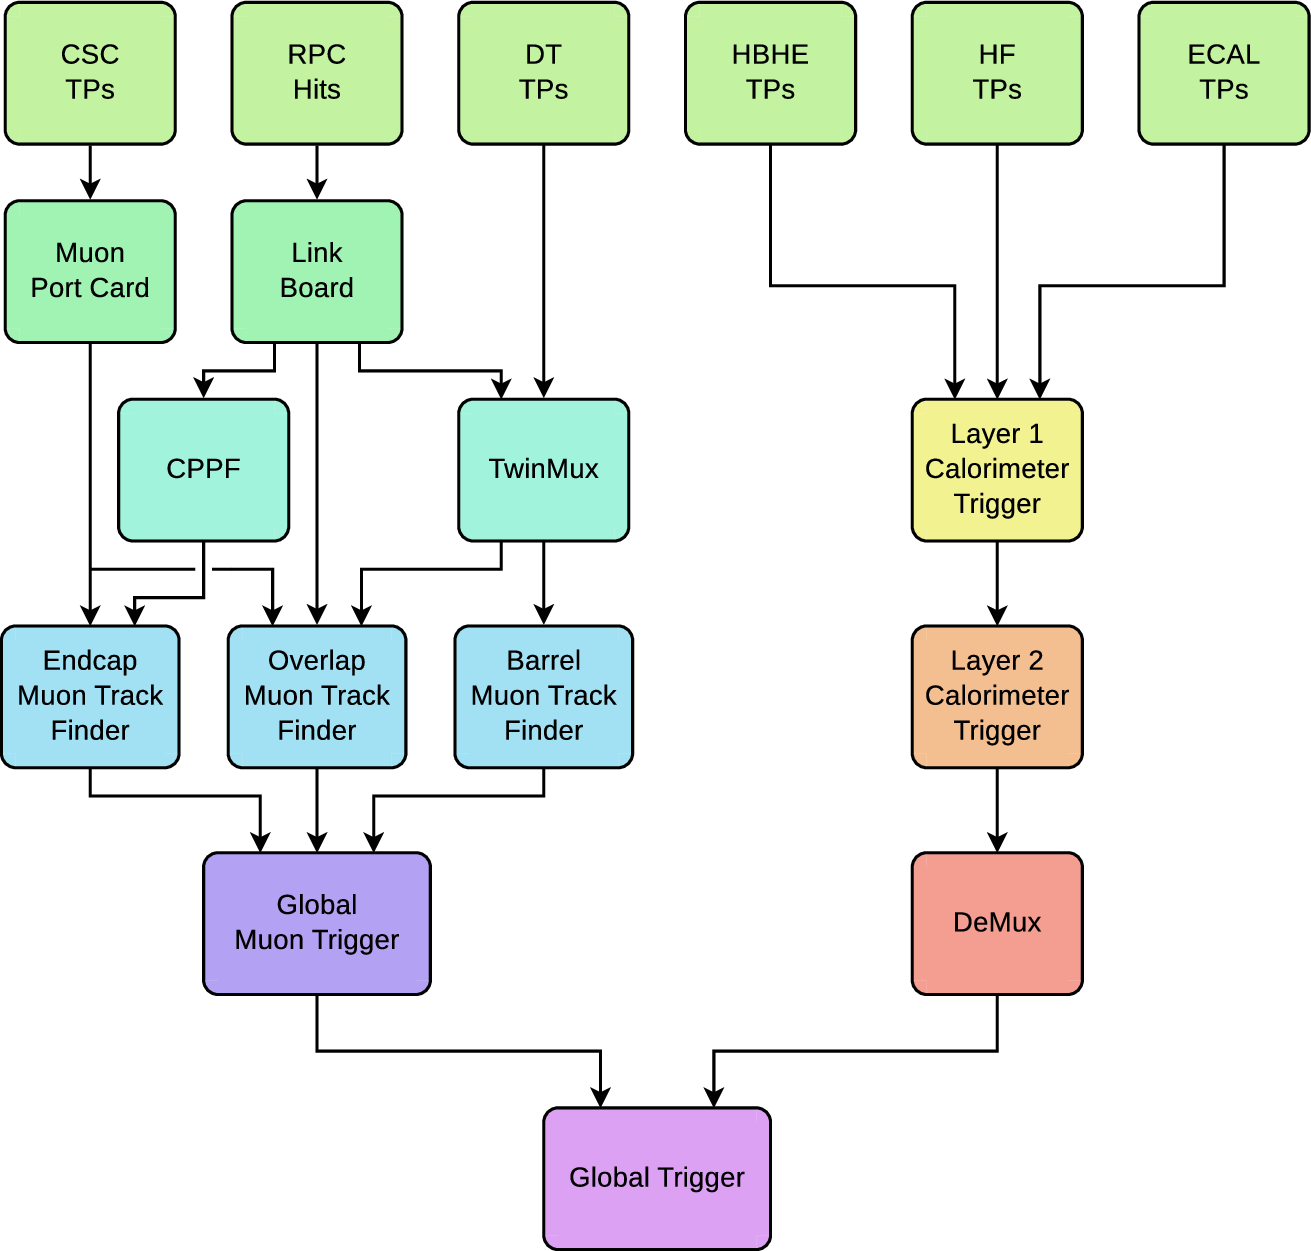
\includegraphics[width=\textwidth]{Images/CMS/L1TriggerMap.png}
    \caption{A flow chart of the CMS L1 trigger system.}
    \label{fig:L1TriggerMap}
\end{figure}

\subsubsection{High-level trigger} \label{sec:HLT}
To further reduce the L1A output rate, the high-level trigger (HLT) makes a final selection of events with a \SI{1}{kHz} readout rate, acceptable for offline reconstruction and permanent storage. Implemented in software running on a farm of commercial computers, the HLT takes an L1A seed and performs a streamlined reconstruction with a similar efficiency to that used in offline processing. The HLT then filters events in roughly two stages: first, using only muon system and calorimeter information, and second, using full tracks. Events selected by the HLT algorithms are sent to permanent storage. A photograph of a GPU used to process the HLT algorithms is shown in Fig.~\ref{fig:HLTGPU}.

\begin{figure}[H]
    \centering
    \includegraphics[width=\textwidth]{Images/CMS/HLTGPU.png}
    \caption{A GPU used to process the HLT algorithms.}
    \label{fig:HLTGPU}
\end{figure}